\documentclass{article}%
\usepackage[T1]{fontenc}%
\usepackage[utf8]{inputenc}%
\usepackage{lmodern}%
\usepackage{textcomp}%
\usepackage{lastpage}%
\usepackage[head=40pt,margin=0.5in,bottom=0.6in]{geometry}%
\usepackage{graphicx}%
%
\title{\textbf{Duque asegura que Colombia no extraditará a Julio Borges}}%
\author{EFE}%
\date{24/09/2018}%
%
\begin{document}%
\normalsize%
\maketitle%
\textbf{URL: }%
http://www.eluniversal.com/politica/21512/duque{-}asegura{-}que{-}colombia{-}no{-}extraditara{-}a{-}julio{-}borges\newline%
%
\textbf{Periodico: }%
EU, %
ID: %
21512, %
Seccion: %
politica\newline%
%
\textbf{Palabras Claves: }%
NO\_TIENE\newline%
%
\textbf{Derecho: }%
1.2, %
Otros Derechos: %
CONTEXTO, %
Sub Derechos: %
1.2.2\newline%
%
\textbf{EP: }%
NO\newline%
\newline%
%
\textbf{\textit{"Nosotros no vamos a extraditar a Julio Borges. Nosotros no vamos a extraditar a un perseguido político para que una dictadura abuse de sus derechos humanos", dijo Duque en declaraciones desde la ONU}}%
\newline%
\newline%
%
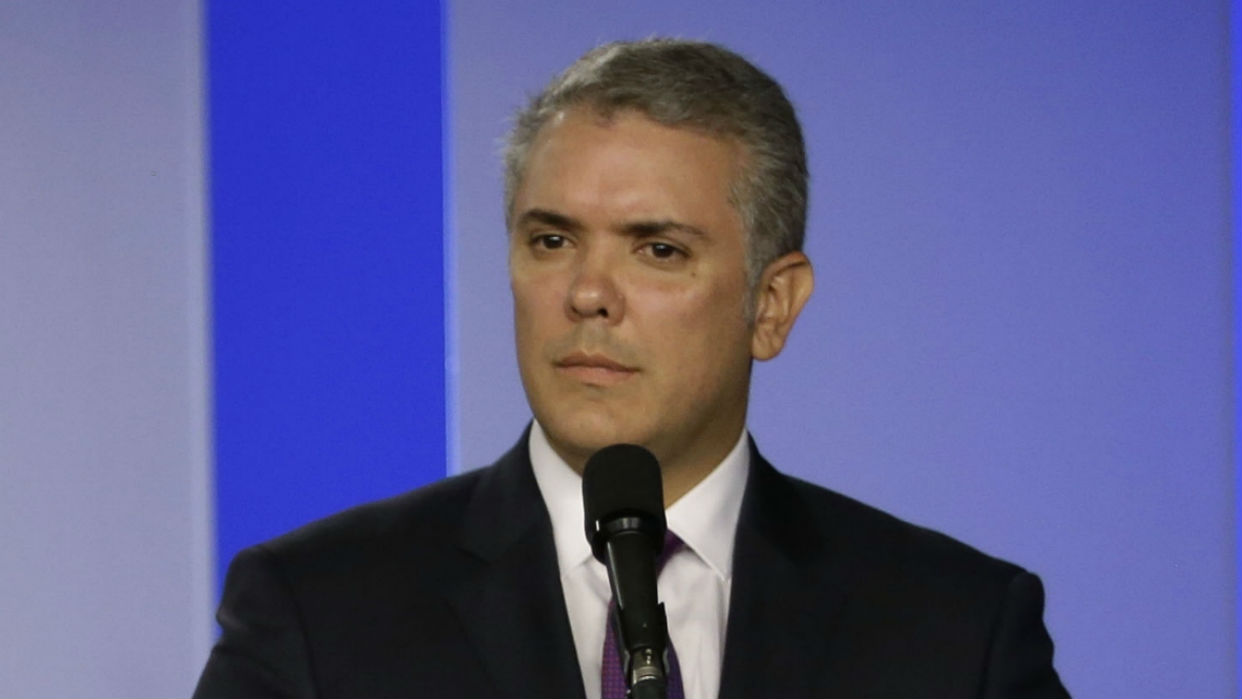
\includegraphics[width=300px]{248.jpg}%
\newline%
%
Naciones Unidas, 24 sep (EFE).{-} El mandatario de Colombia, Iván Duque, aseguró este lunes que su país no va a extraditar a Venezuela al diputado opositor Julio Borges, acusado por un atentado al presidente Nicolás Maduro.%
\newline%
%
"Nosotros no vamos a extraditar a Julio Borges. Nosotros no vamos a extraditar a un perseguido político para que una dictadura abuse de sus derechos humanos", dijo Duque en declaraciones en la sede de Naciones Unidas, reseñó Efe.%
\newline%
%
Según el presidente colombiano, "sería absurdo" pensar en atender la solicitud de Venezuela para la entrega de una "persona que está luchando por las libertades de su pueblo".%
\newline%
%
Duque dijo que su gobierno va a seguir "defendiendo al pueblo venezolano", pidiendo "la libertad de los presos políticos" y demandando "un verdadero y efectivo camino a una transición democrática que le devuelva las libertades" a Venezuela.%
\newline%
%
Este domingo, el Ejecutivo venezolano dijo que estaba a la espera de que Colombia atendiese la solicitud de extradición al considerar que ya estaban presentados todos los elementos para ello.%
\newline%
%
El ministro de Comunicación de Venezuela, Jorge Rodríguez, acusó a Borges de estar detrás del "continuo desencadenamiento de hechos violentos contra Venezuela", entre ellos, mencionó el llamado "golpe azul" en 2015 y por el que hay ocho condenados, cinco de ellos militares.%
\newline%
%
Borges ha negado en reiteradas oportunidades las acusaciones del Gobierno.\newline%
\newline%
El atentado contra Maduro ocurrió el pasado 4 de agosto, cuando el jefe de Estado venezolano presidía un acto con militares en Caracas y dos drones cargados con explosivos detonaron cerca de la tarima presidencial sin causar víctimas fatales.%
\newline%
%
\end{document}